\documentclass{article}


\usepackage{siunitx} % Provides the \SI{}{} and \si{} command for typesetting SI units
\usepackage{graphicx} % Required for the inclusion of images
\usepackage{natbib} % Required to change bibliography style to APA
\usepackage{amsmath} % Required for some math elements 
\usepackage{listings}
\usepackage{placeins}
\usepackage{color}
\setlength\parindent{0pt} % Removes all indentation from paragraphs

\lstset{frame=tb,
  language=Matlab,
  aboveskip=3mm,
  belowskip=3mm,
  showstringspaces=false,
  columns=flexible,
  basicstyle={\small\ttfamily},
  numbers=none,
  numberstyle=\tiny\color{gray},
  keywordstyle=\color{blue},
  commentstyle=\color{green},
  stringstyle=\color{red},
  breaklines=true,
  breakatwhitespace=true,
  tabsize=3}
%\renewcommand{\labelenumi}{\alph{enumi}.} % Make numbering in the enumerate environment by letter rather than number (e.g. section 6)


\title{Lab 5 \\ Binary Data Encoding Systems} % Title

\author{Aneesh Malhotra \\ G00844135} % Author name

\date{\today} % Date for the report

\begin{document}

\maketitle % Insert the title, author and date


% If you wish to include an abstract, uncomment the lines below
% \begin{abstract}
% Abstract text
% \end{abstract}

%----------------------------------------------------------------------------------------
%	SECTION 1
%----------------------------------------------------------------------------------------

\section{Introduction}

\subsection{Objective}
\begin{description}

The objective of this lab is to encode bits using pulses defined by Barker codes, and analyze how we can use the properties of their matched filters to determine the original signal in the presence of noise. 
\end{description}

\subsection{Barker Codes}
Barker codes are signals defined by a sequence of $\pm 1$. Given a pulse $p(t)$, we can encode a binary signal for which at every time period $T_p$, the pulse $p(t)$ represents a 1 and the pulse $-p(t)$ represents a zero. Barker codes minimize the autocorrelation of a function, so that if it is convolved with its matched filter we see very little energy in the output until a complete overlap, at which case the energy is maximized, giving us a sharp spike.  If Barker Codes are used to represent the pulse $p(t)$, we can take an encoded signal $s(t)$ and pass it through the Barker Codes' matched filter. This would minimize the output at every point except for complete overlaps, at which point we would see either a positive or negative spike, representing either a $1$ or a $0$. This would allow us to encode the input message by looking at each spike. There are only 7 known Barker Codes, corresponding to sequences of $1$ and $-1$ of lengths 2, 3, 4, 5, 7, 11, and 13. Barker Codes are used particularly for communication, namely radar, since they allow us to easily detect pulses. Finally, Barker Codes are very good for handling Gaussian noise. If a signal defined by Barker Codes goes through a noisy channel, the matched filter will minimize the noise in the output, and maximize the spike.

%---------------------------------------------------------------------------------------- 
%	SECTION 2
%----------------------------------------------------------------------------------------

\section{Main Body}

\subsection{Part 1}
First we analyzed matched filters of pulses $p_3(t)$ and $p_11(t)$, which represent the Barker Codes [1, 1, -1] and [1, 1, 1, -1, -1, -1, 1, -1, -1, 1, -1]. We passed these functions through their matched filters, whose impulse response is given by their causal time reversal $p_(T_p - t)$ The plots of $p_3$ and $p_11$ with their matched filters is shown below.
\begin{figure}[!htb]
    \centering
    \begin{minipage}{.5\textwidth}
        \centering
        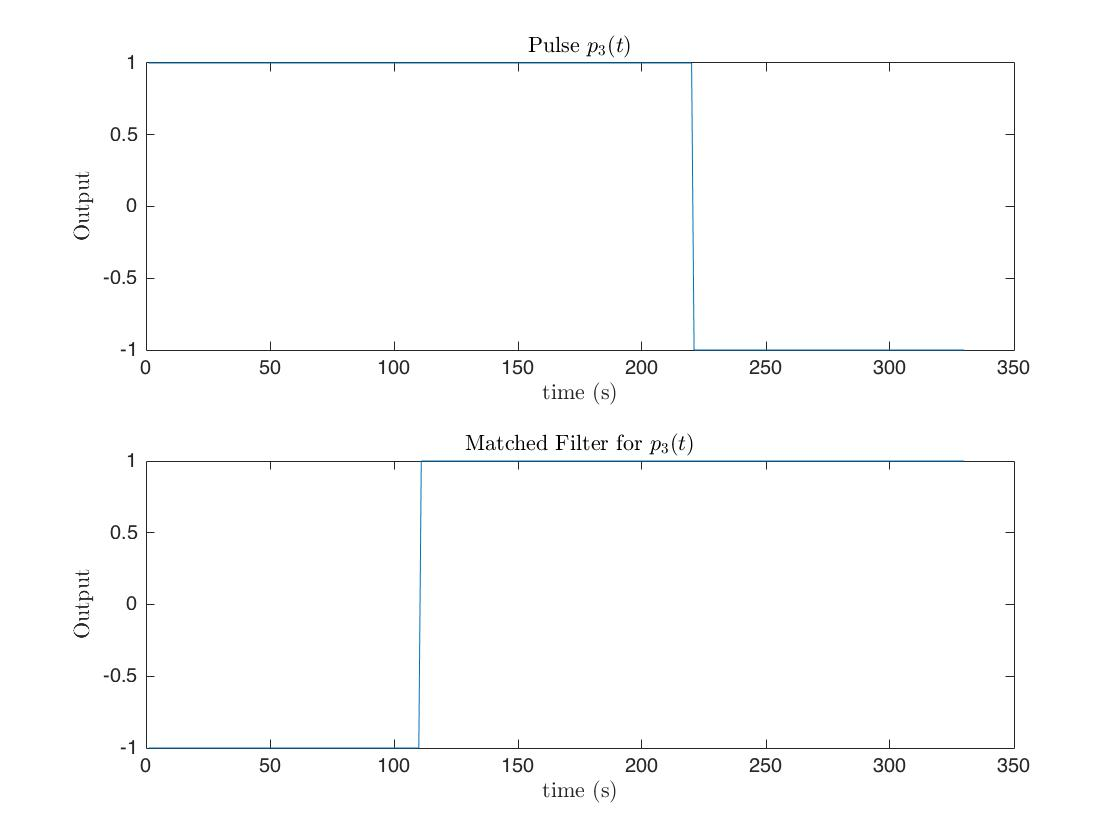
\includegraphics[width=1.0\linewidth, height=0.2\textheight]{p3.jpg}
        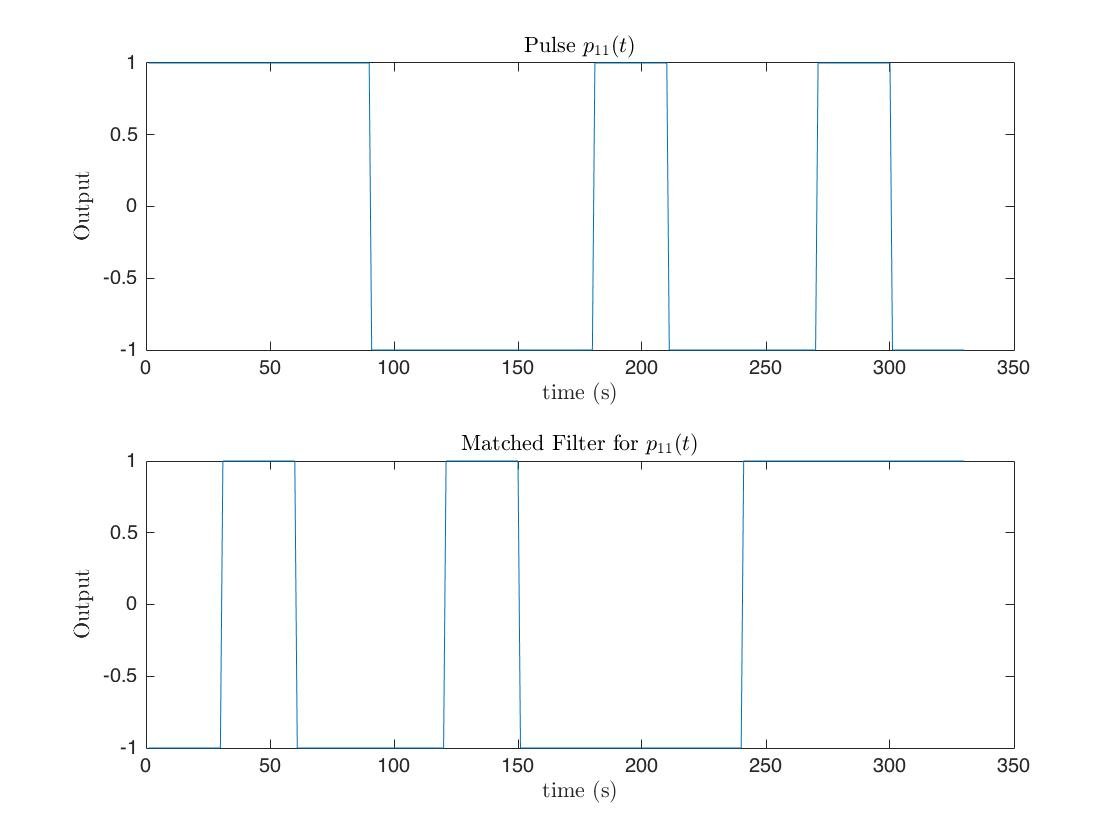
\includegraphics[width=1\linewidth, height=0.2\textheight]{p11.jpg}
    \end{minipage}
    \caption{Pulses $p_3$ and $p_11$ with their matched filters}
\end{figure}
\FloatBarrier
We then found the outputs of the matched filters by convolution and obtained the following plots:
\begin{figure}[!htb]
    \centering
    \begin{minipage}{.5\textwidth}
        \centering
        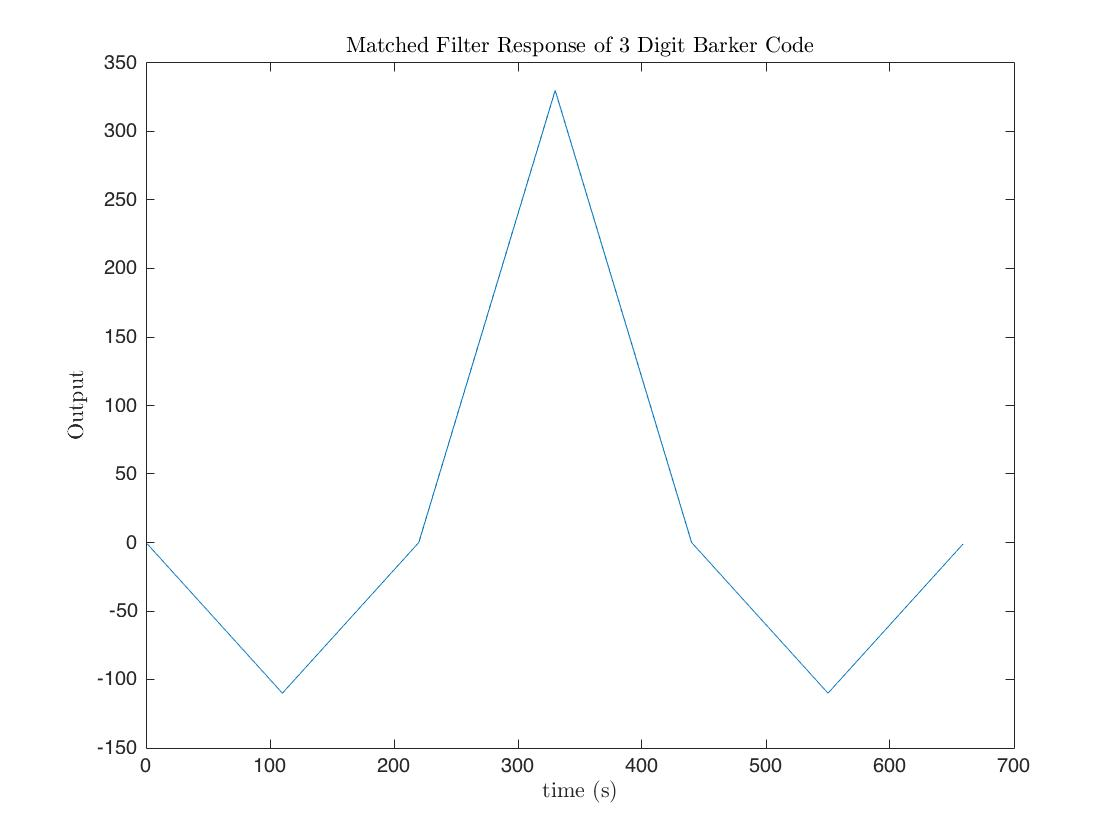
\includegraphics[width=1.0\linewidth, height=0.2\textheight]{match3.jpg}

        \label{fig:prob1_6_2}
    \end{minipage}%
    \begin{minipage}{0.5\textwidth}
        \centering
        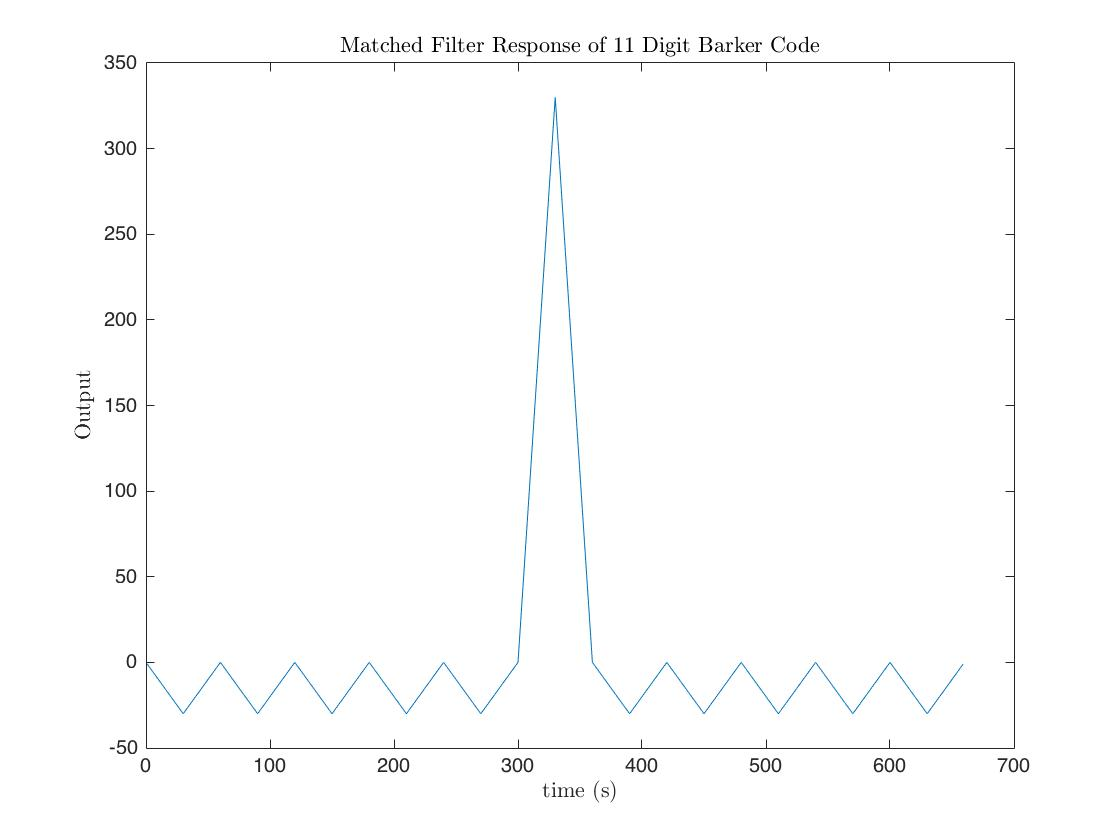
\includegraphics[width=1\linewidth, height=0.2\textheight]{match11.jpg}

        \label{fig:prob1_6_1}
    \end{minipage}
    \caption{Output of $h_{MF3}*p_3$ and $h_{MF11}*p_{11}}
\end{figure}

\clearpage
We see that the output of each of the filters is a spike at the the point where there is complete overlap. This occurs at $T_p = 330$. The maximum output is also 330. 

\subsection{Part 2}
In this section we created a discrete Gaussian noise signal of length 100, called SIG by taking the sign of a random noise signal. We then defined the signals $s_3$ to be $p_3$ at every $nT_p$ seconds if the $n$th value of SIG is 1 and $-p_3(t)$ if the $n$th value of SIG is positive. This creates a signal of $33,000$ samples containing either $p_3$ or $-p_3$ at every $330$ samples. We repeated this for $p_{11}$ to create $s_{11}$. The plots of the first 4 bits of each is shown below. 


\begin{figure}[!htb]
    \centering
    \begin{minipage}{.5\textwidth}
        \centering
        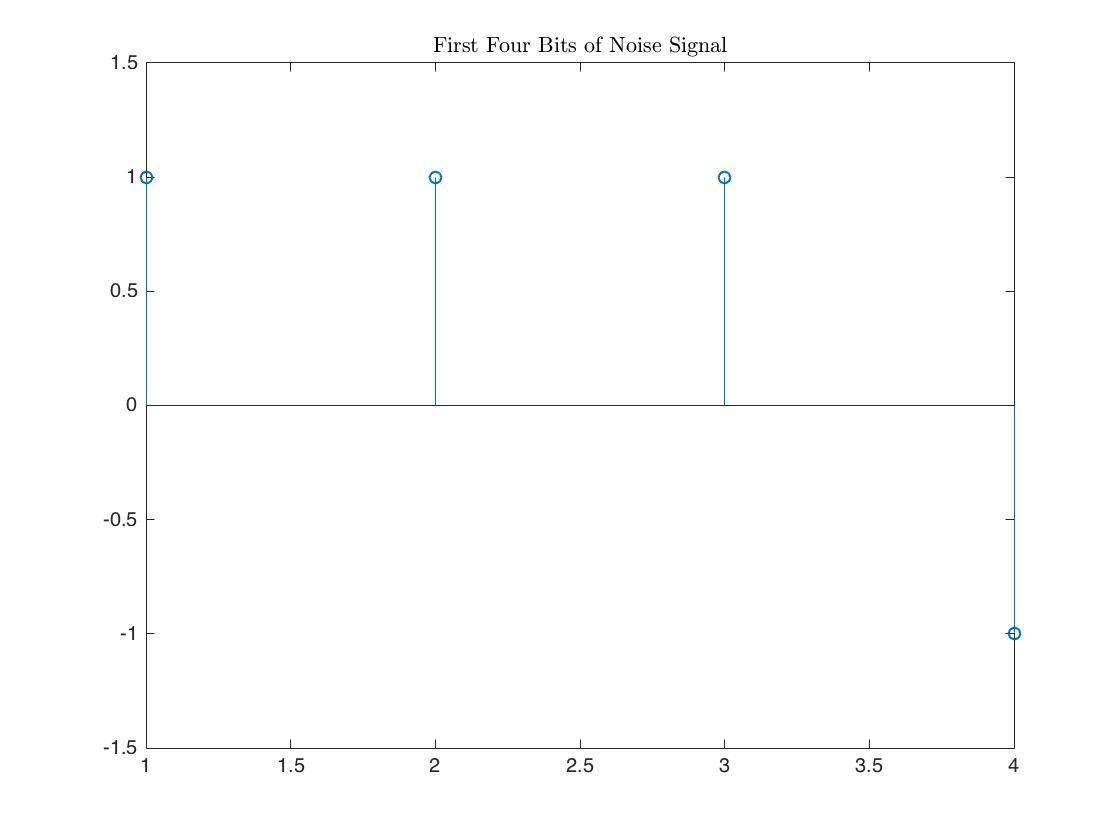
\includegraphics[width=1.0\linewidth, height=0.2\textheight]{noise.jpg}

        \label{fig:prob1_6_2}
    \end{minipage}
    \caption{First 4 bits of SIG}
\end{figure}

\begin{figure}[!htb]
    \centering
    \begin{minipage}{.5\textwidth}
        \centering
        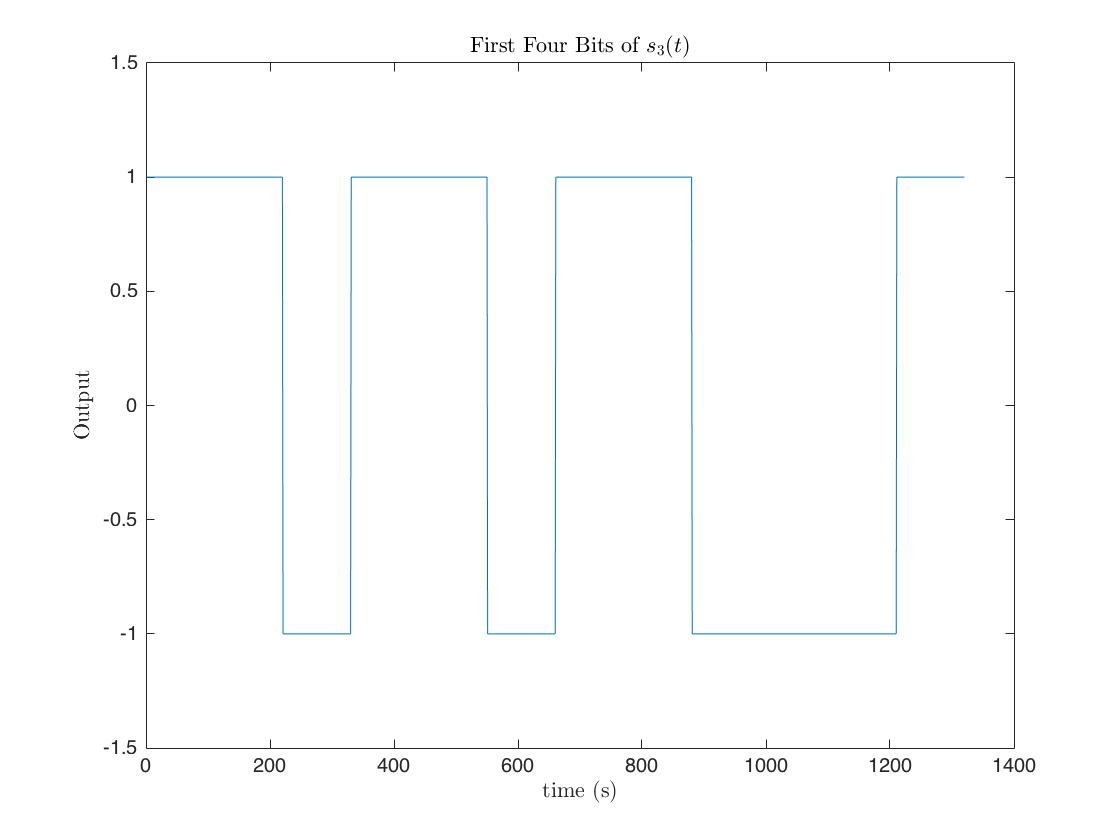
\includegraphics[width=1.0\linewidth, height=0.2\textheight]{s3.jpg}

        \label{fig:prob1_6_2}
    \end{minipage}%
    \begin{minipage}{0.5\textwidth}
        \centering
        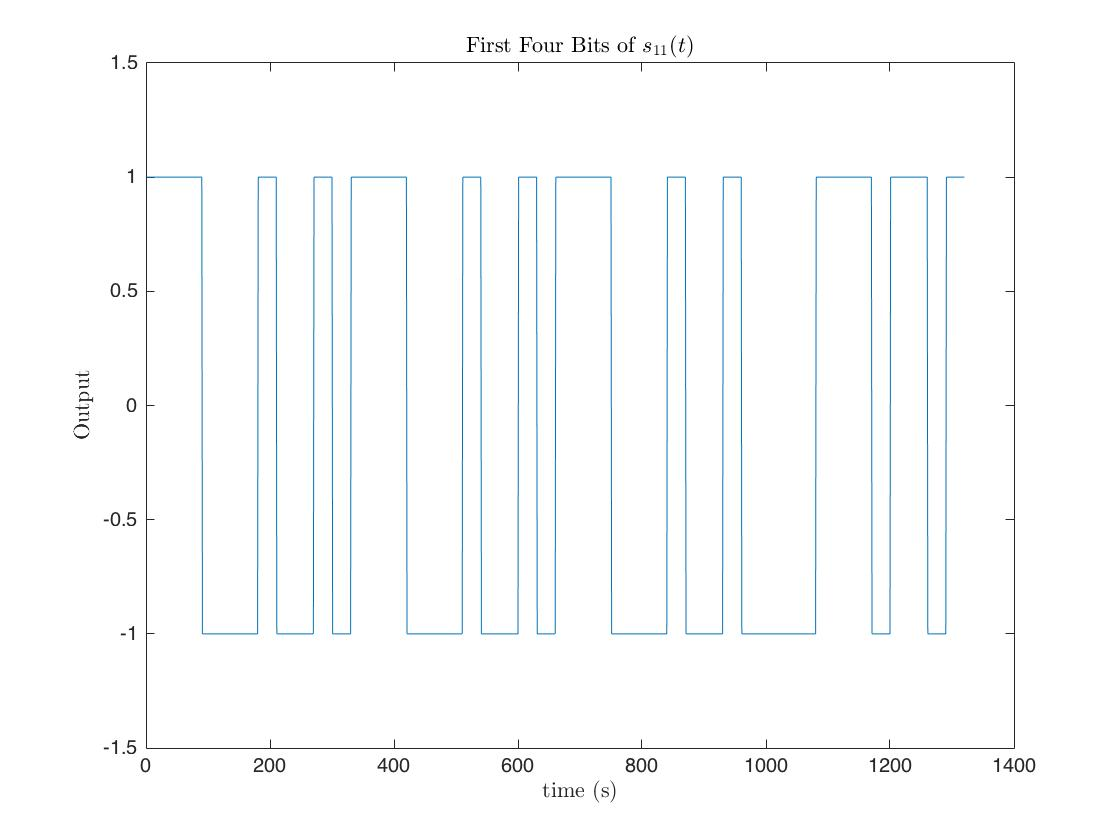
\includegraphics[width=1\linewidth, height=0.2\textheight]{s11.jpg}

        \label{fig:prob1_6_1}
    \end{minipage}
    \caption{First 4 time periods of $s_11$ and $s_3$}
\end{figure}






\subsection{Part 3}
In this section we defined a Gaussian Noise signal $nse$ and added it to the signals defined in the previous section

\begin{align*}
x_1(t) = s_3(t) + nse \\
x_3(t) = s_3(t) + 3nse \\ 
x_5(t) = s_5(t) + 5nse.
\end{align*}
We then found the output of these signals with both matched filter $h_{MF3}$ and $h_{MF11}$. This was repeated for $s_{11}(t)$. The plots are shown below:

\begin{figure}[!htb]
    \centering
    \begin{minipage}{.5\textwidth}
        \centering
        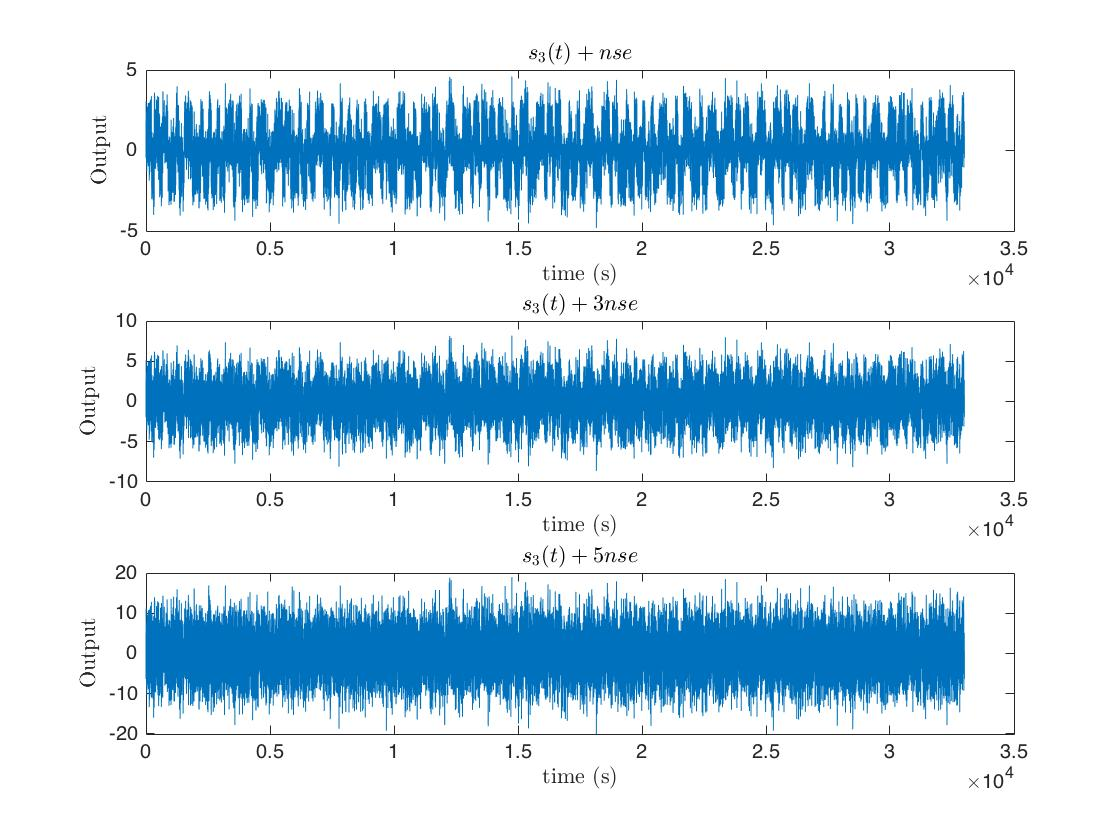
\includegraphics[width=1.0\linewidth, height=0.2\textheight]{s3noise.jpg}

        \label{fig:prob1_6_2}
    \end{minipage}
    \caption{Noisy $s_3$ signal}
\end{figure}

\begin{figure}[!htb]
    \centering
    \begin{minipage}{.5\textwidth}
        \centering
        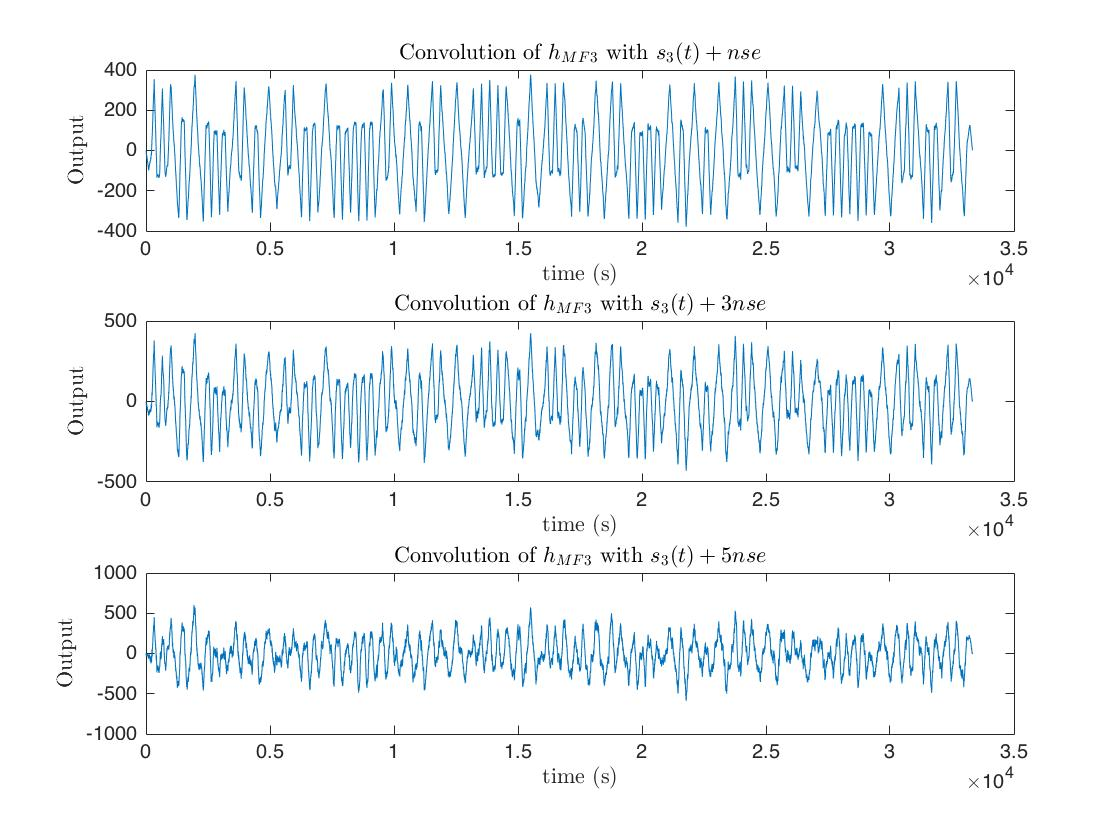
\includegraphics[width=1.0\linewidth, height=0.2\textheight]{s3h3.jpg}

        \label{fig:prob1_6_2}
    \end{minipage}
    \caption{Noisy $s_3$ through the correct matched filter}
\end{figure}

\begin{figure}[!htb]
    \centering
    \begin{minipage}{.5\textwidth}
        \centering
        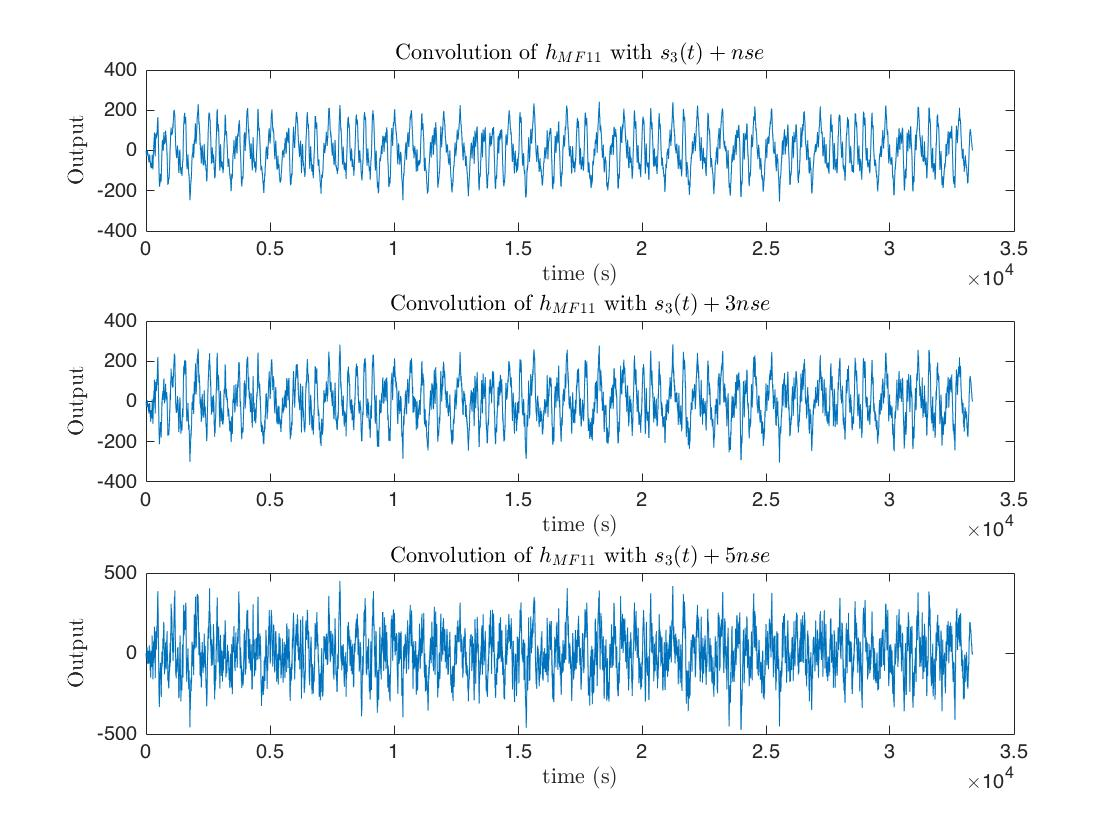
\includegraphics[width=1.0\linewidth, height=0.2\textheight]{s3h11.jpg}

        \label{fig:prob1_6_2}
    \end{minipage}
    \caption{Noisy $s_3$ through the incorrect matched filter}
\end{figure}


\begin{figure}[!htb]
    \centering
    \begin{minipage}{.5\textwidth}
        \centering
        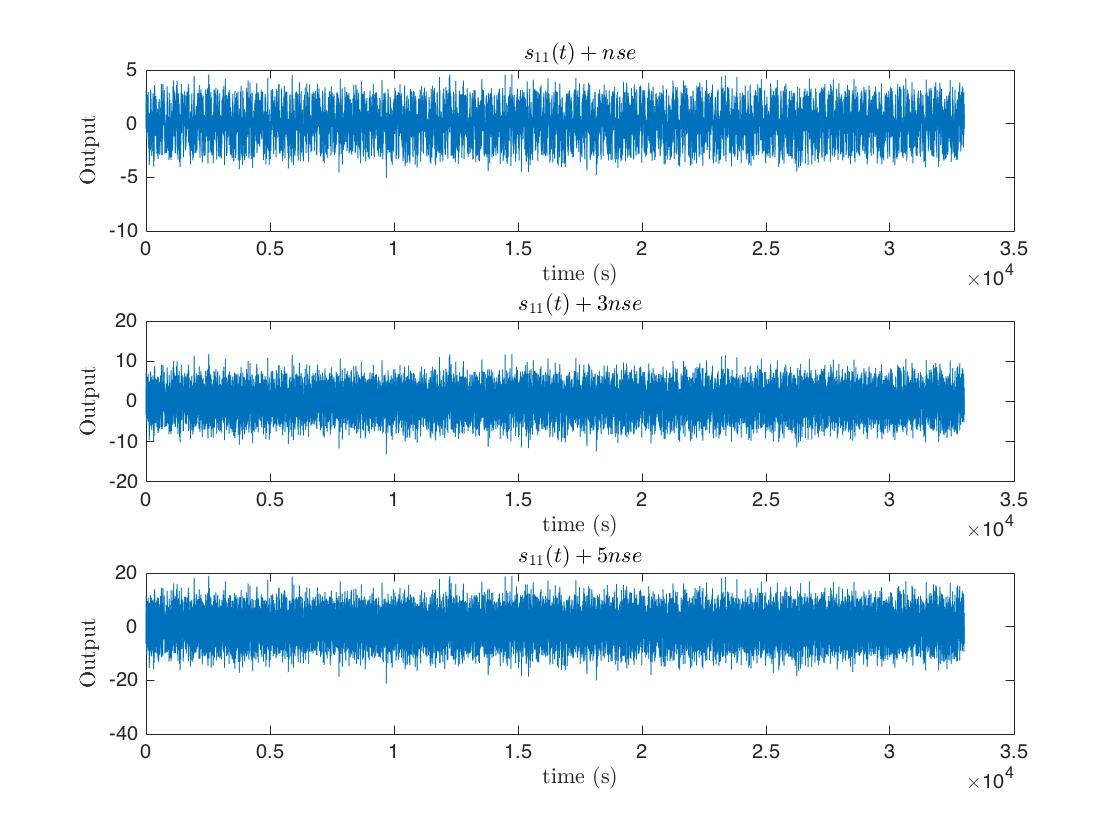
\includegraphics[width=1.0\linewidth, height=0.2\textheight]{s11noise.jpg}

        \label{fig:prob1_6_2}
    \end{minipage}
    \caption{Noisy $s_{11}$ signal}
\end{figure}

\begin{figure}[!htb]
    \centering
    \begin{minipage}{.5\textwidth}
        \centering
        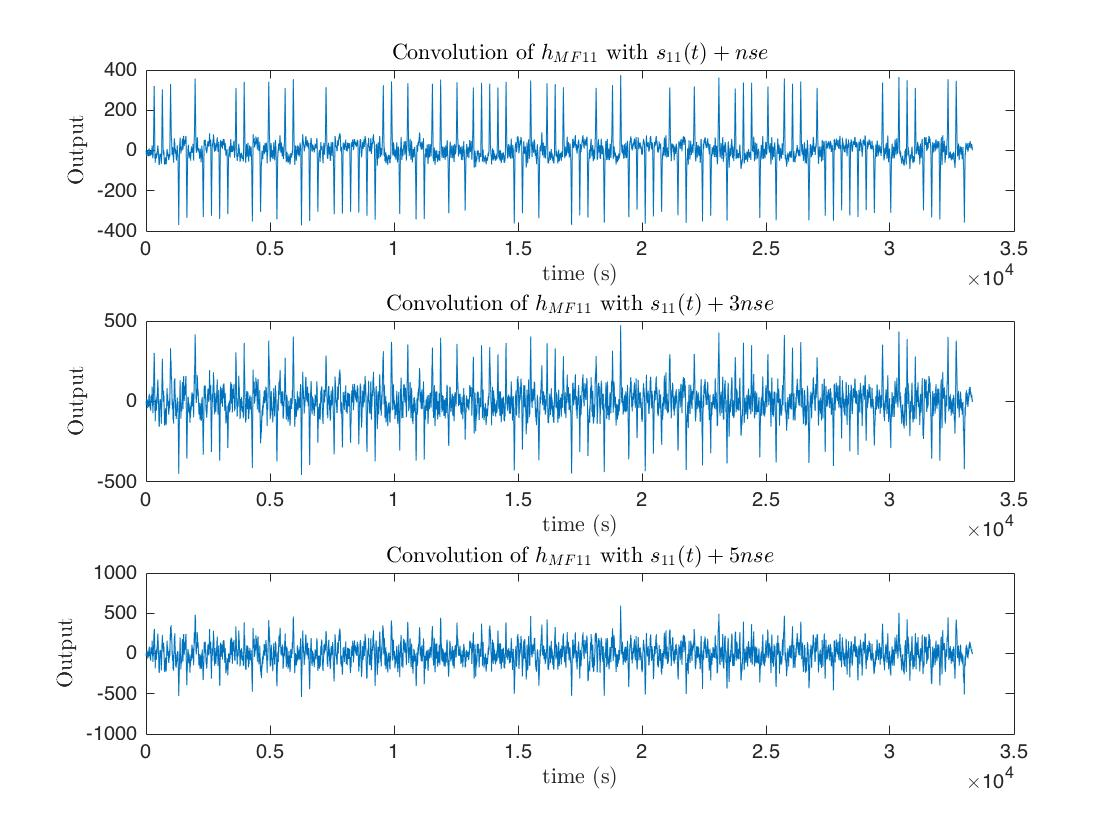
\includegraphics[width=1.0\linewidth, height=0.2\textheight]{s11h11.jpg}

        \label{fig:prob1_6_2}
    \end{minipage}
    \caption{$s_{11}$ through the correct matched filter}
\end{figure}

\begin{figure}[!htb]
    \centering
    \begin{minipage}{.5\textwidth}
        \centering
        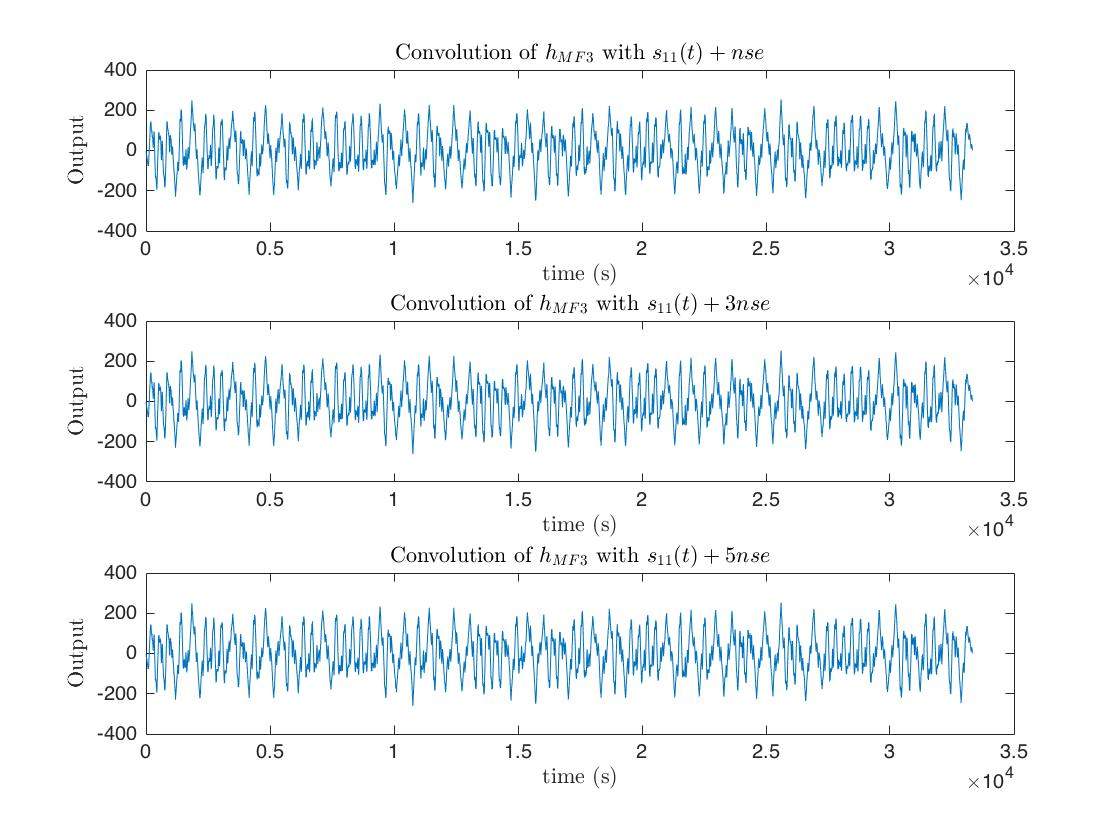
\includegraphics[width=1.0\linewidth, height=0.2\textheight]{s11h3.jpg}

        \label{fig:prob1_6_2}
    \end{minipage}
    \caption{$s_{11}$ through incorrect matched filter}
\end{figure}

\FloatBarrier
We see that in each case, the correct matched filter clearly shows the bits, whereas using the other matched filter makes it more difficult to identify the bits 

%----------------------------------------------------------------------------------------
%	SECTION 4
%----------------------------------------------------------------------------------------
\FloatBarrier
\section{Conclusion}
In this lab we saw how to send binary signals using continuous waveforms by using Barker Codes. Barker Codes allowed us to create pulses that are orthogonal when they overlap, creating an output signal with far more energy at their overlap point $T_p$ than at every other point. By sending messages encoded with Barker Codes, we can identify the spikes, and therefore the Boolean value of the signal at each time period, allowing us to decode messages easily. We saw that this was even true for signals with Gaussian noise. The signals with low noise were easily detectable. While the signal with the highest noise $s_11 + 5nse$ was still mostly readable, there were still some ambiguities about where spikes were. This was likely due to the noise being in high enough magnitude to swamp the original signal, making the output from the matched filter far less readable. Finally, we saw that by using the incorrect matched filter, there were many more ambiguities about the input signal, as the spikes were very poorly defined and many spikes corresponded to incorrect bits. This shows the precision of the spikes in the convolution of the Barker Codes with their matched filter and how using the incorrect filter can make the input unreadable. 
\section{Appendix}

\subsection{Code}
\lstinputlisting{lab5.m}



%----------------------------------------------------------------------------------------
%	BIBLIOGRAPHY
%----------------------------------------------------------------------------------------
\section{References}
\begin{enumerate}
\item Lathi, B. P. Linear Systems and Signals. New York: Oxford UP, 2005. Print.

\item Ranganath, P., & Rao, S. (2014). Effect of Pulse Shaping on Autocorrelation Function of Barker and Frank Phase Codes. Journal of Advanced Electrical and Computer Engineering, 1(1), 22-31.
\end{enumerate}
\end{document}